% ===========================================================================
% Section 6 — Experimental Results
% ===========================================================================

\section{Experimental Results}
\label{sec:results}

% ---------------------------------------------------------------------------
\subsection{Experimental Setup}
\label{sec:setup}

\subsubsection{Dataset}
The NIST Juliet Test Suite for C/C++ v1.3~\cite{juliet2017} was used as the
primary dataset.  After parsing and preprocessing, the dataset comprises
\textbf{105,183} source code samples spanning \textbf{118}~CWE categories.
The template-aware splitting strategy (Section~\ref{sec:data_design})
produced:
\begin{itemize}
    \item \textbf{Training set:} 82,736 samples across 118~CWE categories
          and 1,323 unique templates.
    \item \textbf{Test set:} 22,447 samples across 87~CWE categories
          and 366 unique templates.
\end{itemize}
The 31~CWE categories absent from the test set contain only a single
template each; these are assigned entirely to the training set to prevent
information loss, as described in Section~\ref{sec:data_design}.
Zero template overlap exists between the training and test sets.

\subsubsection{Hardware Environment}
All experiments were conducted on a laptop workstation with the
specifications listed in Table~\ref{tab:hardware}.

\begin{table}[t]
\centering
\caption{Hardware environment for all experiments.}
\label{tab:hardware}
\begin{tabular}{ll}
\hline
\textbf{Component}    & \textbf{Specification} \\
\hline
Processor             & 13th Gen Intel Core i7-13850HX @ 2.10\,GHz \\
Cores / Threads       & 20 cores / 28 logical processors \\
GPU                   & NVIDIA RTX 2000 Ada Generation (Laptop) \\
VRAM                  & 8\,GB (7,957\,MB) \\
System Memory         & DDR5 \\
\hline
\end{tabular}
\end{table}

\subsubsection{Software and Frameworks}
The implementation uses Python~3.13 with the software stack detailed in
Table~\ref{tab:software}.  All models were loaded via the Hugging Face
Transformers library.  Quantisation for zero-shot and QLoRA models used
\texttt{bitsandbytes} with NF4 4-bit encoding.

\begin{table}[t]
\centering
\caption{Software frameworks and versions.}
\label{tab:software}
\begin{tabular}{ll}
\hline
\textbf{Framework}        & \textbf{Version} \\
\hline
PyTorch                    & $\geq$ 2.0.0 \\
Hugging Face Transformers  & $\geq$ 5.5.4 \\
PEFT (LoRA / QLoRA)        & $\geq$ 0.15.0 \\
scikit-learn               & $\geq$ 1.3.0 \\
bitsandbytes               & $\geq$ 0.43.0 \\
Hugging Face Accelerate    & $\geq$ 0.27.0 \\
Streamlit (UI)             & $\geq$ 1.30.0 \\
TensorBoard (logging)      & $\geq$ 2.14.0 \\
\hline
\end{tabular}
\end{table}

\subsubsection{Hyperparameters}
Table~\ref{tab:hyperparams} summarises the hyperparameters used for the
two training paradigms.  All fine-tuned encoder models share the same
hyperparameter configuration.  The QLoRA configuration was designed
specifically for the 8\,GB VRAM constraint.

\begin{table}[t]
\centering
\caption{Hyperparameter settings for encoder and QLoRA training.}
\label{tab:hyperparams}
\begin{tabular}{lcc}
\hline
\textbf{Hyperparameter} & \textbf{Encoder Models} & \textbf{QLoRA} \\
\hline
Learning rate            & $5 \times 10^{-5}$      & $2 \times 10^{-4}$ \\
Optimiser                & AdamW                   & PagedAdamW (8-bit) \\
Weight decay             & 0.01                    & 0.01 \\
Batch size               & 8                       & 2 \\
Gradient accumulation    & 1                       & 4 \\
Effective batch size     & 8                       & 8 \\
Max sequence length      & 256 tokens              & 256 tokens \\
Epochs                   & 2                       & 5 \\
Early stopping patience  & 1 epoch                 & 2 epochs \\
Dropout                  & 0.1                     & 0.05 (LoRA) \\
Precision                & FP16                    & BF16 \\
Loss function            & Cross-entropy           & Cross-entropy \\
Seed                     & 42                      & 42 \\
\hline
\end{tabular}
\end{table}

% ---------------------------------------------------------------------------
\subsection{Performance Evaluation}
\label{sec:performance}

\subsubsection{Overall Model Comparison}
Table~\ref{tab:model_comparison} presents the comprehensive evaluation of
all six model configurations on the test set.  All metrics are
macro-averaged across the 118~CWE classes.

\begin{table*}[t]
\centering
\caption{Comprehensive model comparison on the Juliet C/C++ v1.3 test set.
         All classification metrics are macro-averaged.  Inference latency
         is the mean over 20~forward passes after a 5-run warmup with CUDA
         synchronisation.  Zero-shot models are evaluated on random subsets
         (sample counts noted) due to high per-sample inference cost.}
\label{tab:model_comparison}
\begin{tabular}{lccccccccc}
\hline
\textbf{Model} &
\textbf{Params} &
\textbf{Size} &
\textbf{Accuracy} &
\textbf{Precision} &
\textbf{Recall} &
\textbf{F1} &
\textbf{MCC} &
\textbf{FPR} &
\textbf{Latency} \\
& & (MB) & & & & & & & (ms) \\
\hline
\multicolumn{10}{l}{\textit{Fine-tuned encoder models (full test set, 22,447 samples)}} \\
\hline
CodeT5-Small        & 35.4\,M  & 404.9   & 0.9980 & 0.9533 & 0.9534 & 0.9533 & 0.9979 & 1.80$\times 10^{-5}$ & 17.2 \\
\textbf{CodeT5-Base}& 109.7\,M & 1,255.5 & 0.9978 & 0.9585 & 0.9644 & \textbf{0.9605} & 0.9977 & 1.92$\times 10^{-5}$ & 24.9 \\
CodeBERT-Base       & 124.7\,M & 1,423.2 & 0.9963 & 0.9574 & 0.9539 & 0.9512 & 0.9961 & 3.33$\times 10^{-5}$ & 19.4 \\
GraphCodeBERT-Base  & 124.7\,M & 1,423.2 & 0.9975 & 0.9530 & 0.9530 & 0.9530 & 0.9974 & 2.23$\times 10^{-5}$ & 26.9 \\
\hline
\multicolumn{10}{l}{\textit{Zero-shot generative models (sampled subsets)}} \\
\hline
CodeGemma-2B (ZS)\textsuperscript{a}    & 2.51\,B  & 4,677 & 0.2500 & 0.1755 & 0.0832 & 0.0948 & 0.3022 & 6.89$\times 10^{-3}$ & 3,277 \\
Gemma-4-E2B-IT (ZS)\textsuperscript{b}  & 5.13\,B  & 9,561 & 0.7800 & 0.6990 & 0.7167 & 0.6988 & 0.7799 & 2.00$\times 10^{-3}$ & 396,273 \\
\hline
\multicolumn{10}{l}{\footnotesize\textsuperscript{a}~500 samples. \textsuperscript{b}~50 samples.} \\
\end{tabular}
\end{table*}

The four fine-tuned encoder models all achieve test accuracy above 99.6\%
and macro-F1 scores exceeding 0.95.  \textbf{CodeT5-Base} achieves the
highest macro-F1 of \textbf{0.9605}, outperforming the larger
CodeBERT-Base (125\,M parameters) despite having fewer parameters
(110\,M).  This result suggests that the T5 encoder's bimodal pre-training
on code and natural language produces superior representations for CWE
classification compared to the RoBERTa-based architecture.

The Matthews Correlation Coefficient (MCC) values for all fine-tuned models
exceed 0.996, confirming strong classification performance that is robust
to any class imbalance.  The macro False Positive Rate (FPR) remains below
$3.4 \times 10^{-5}$ across all fine-tuned models, indicating negligible
false alarm rates per class.

\subsubsection{Zero-Shot vs.\ Fine-Tuned Performance}
The zero-shot models demonstrate a substantial performance gap compared to
fine-tuned models.  CodeGemma-2B achieves only 25.0\% accuracy and
0.0948~macro-F1 on 500 samples, performing only marginally above random
chance for 118~classes (expected $\approx 0.85\%$).  Gemma-4-E2B-IT, an
instruction-tuned model with 5.13\,B parameters (2.3\,B effective),
achieves considerably better zero-shot performance at 78.0\% accuracy and
0.6988~macro-F1 on 50~samples, demonstrating the benefit of
instruction-tuning for structured classification tasks.

However, even the best zero-shot model falls short of fine-tuned
performance by \textbf{28.1 percentage points} in accuracy and
\textbf{0.2617} in macro-F1, while requiring $\mathbf{15{,}600\times}$
longer inference time per sample (396\,s vs.\ 25\,ms for CodeT5-Base).
This result strongly motivates parameter-efficient fine-tuning approaches
such as QLoRA for larger models.

\subsubsection{Training Convergence and Early Stopping}
Table~\ref{tab:convergence} presents the per-epoch training dynamics for
the fine-tuned encoder models.  All models converge rapidly, achieving peak
performance within 1--2~epochs on this dataset.

\begin{table}[t]
\centering
\caption{Per-epoch test metrics and training convergence.  Bold values
         indicate the best epoch selected by early stopping on macro-F1.}
\label{tab:convergence}
\begin{tabular}{lccccc}
\hline
\textbf{Model} & \textbf{Epoch} & \textbf{Test Loss} & \textbf{Acc.} & \textbf{F1} & \textbf{Time} \\
\hline
CodeT5-Small      & \textbf{1} & \textbf{---}  & ---   & ---   & ---  \\
                  & \textbf{2} & \textbf{0.0102} & \textbf{0.9980} & \textbf{0.9533} & 53\,min \\
\hline
CodeT5-Base       & \textbf{1} & \textbf{---}  & ---   & ---   & ---  \\
                  & \textbf{2} & \textbf{0.0090} & \textbf{0.9978} & \textbf{0.9605} & 53\,min \\
\hline
CodeBERT-Base     & \textbf{1} & \textbf{0.0212} & \textbf{0.9963} & \textbf{0.9512} & 22\,min \\
                  & 2 & 0.0148 & 0.9971 & 0.9377 & 43\,min \\
\hline
GraphCodeBERT     & \textbf{1} & \textbf{0.0114} & \textbf{0.9975} & \textbf{0.9530} & 23\,min \\
                  & 2 & 0.0361 & 0.9928 & 0.8952 & 43\,min \\
\hline
\end{tabular}
\end{table}

A notable finding is the \emph{overfitting behaviour} of CodeBERT-Base and
GraphCodeBERT-Base at epoch~2.  GraphCodeBERT's macro-F1 drops from
0.9530 to 0.8952 (a decrease of \textbf{5.78 percentage points}), and its
test loss increases from 0.0114 to 0.0361 --- a clear sign of overfitting.
CodeBERT similarly degrades from 0.9512 to 0.9377 in F1 despite a decrease
in test loss, indicating growing confusion among minority CWE classes.
Early stopping at patience~$= 1$ effectively mitigates this issue,
selecting the epoch-1 checkpoint for both models.

In contrast, the CodeT5 family continues to improve through epoch~2,
suggesting that the T5 encoder architecture generalises more robustly on
code vulnerability classification tasks.

\subsubsection{Training Efficiency}
Table~\ref{tab:training_time} compares the total training time and
resource requirements across all model configurations.

\begin{table}[t]
\centering
\caption{Training time and resource comparison.}
\label{tab:training_time}
\begin{tabular}{lccc}
\hline
\textbf{Model} & \textbf{Params} & \textbf{Time} & \textbf{Best Epoch} \\
\hline
CodeT5-Small       & 35.4\,M  & 53\,min & 2 \\
CodeT5-Base        & 109.7\,M & 53\,min & 2 \\
CodeBERT-Base      & 124.7\,M & 43\,min & 1 \\
GraphCodeBERT-Base & 124.7\,M & 43\,min & 1 \\
\hline
CodeGemma-2B (QLoRA)\textsuperscript{*} & 2.51\,B & In progress & --- \\
CodeGemma-2B (ZS)  & 2.51\,B  & N/A   & --- \\
Gemma 4 E2B IT (ZS)& 5.13\,B  & N/A   & --- \\
\hline
\multicolumn{4}{l}{\footnotesize\textsuperscript{*}QLoRA trains only $\approx$0.5\% of parameters.} \\
\end{tabular}
\end{table}

All fine-tuned encoder models complete training in under 53~minutes on the
8\,GB VRAM GPU, demonstrating the feasibility of vulnerability detection
model development on consumer-grade hardware.  The RoBERTa-family models
(CodeBERT, GraphCodeBERT) train faster per epoch ($\approx$22\,min) than the
T5-family ($\approx$27\,min), but converge one epoch earlier, resulting in
comparable total wall-clock times.

\subsubsection{Error Analysis}
To understand the failure modes of the best-performing model (CodeT5-Base),
we analyse its per-class performance and the most frequently confused CWE
pairs.

\paragraph{Per-class performance.}
Of the 87~CWE categories present in the test set, \textbf{74~categories
(85.1\%)} achieve perfect F1 scores of 1.00.  Only three categories produce
F1 scores of 0.00: CWE-561 (Dead Code), CWE-562 (Return of Stack Variable
Address), and CWE-674 (Uncontrolled Recursion).  Notably, each of these
categories has only \textbf{1~sample} in the test set, making reliable
evaluation infeasible.  The weighted macro-F1 of \textbf{0.9979} confirms
that the model performs accurately on the vast majority of samples.

\paragraph{Confusion analysis.}
Table~\ref{tab:confusion_pairs} lists the most frequently confused CWE
pairs.  The dominant error pattern involves misclassifications towards
CWE-126 (Buffer Over-read) and CWE-127 (Buffer Under-read).

\begin{table}[t]
\centering
\caption{Top-10 most frequently confused CWE pairs for CodeT5-Small
         (evaluated on full test set of 22,447 samples).}
\label{tab:confusion_pairs}
\begin{tabular}{llc}
\hline
\textbf{Actual CWE} & \textbf{Predicted CWE} & \textbf{Count} \\
\hline
CWE-114 (Process Control)         & CWE-126 (Buffer Over-read) & 8 \\
CWE-194 (Sign Extension)          & CWE-126 (Buffer Over-read) & 6 \\
CWE-90  (LDAP Injection)          & CWE-127 (Buffer Under-read)& 4 \\
CWE-121 (Stack Buffer Overflow)   & CWE-126 (Buffer Over-read) & 4 \\
CWE-123 (Write-what-where)        & CWE-126 (Buffer Over-read) & 4 \\
CWE-366 (Race Condition)          & CWE-126 (Buffer Over-read) & 4 \\
CWE-191 (Integer Underflow)       & CWE-126 (Buffer Over-read) & 3 \\
CWE-511 (Logic/Time Bomb)         & CWE-126 (Buffer Over-read) & 3 \\
CWE-23  (Path Traversal)          & CWE-127 (Buffer Under-read)& 2 \\
CWE-483 (Block Delimitation)      & CWE-126 (Buffer Over-read) & 2 \\
\hline
\end{tabular}
\end{table}

The concentration of misclassifications towards CWE-126 (23 of 40 total
errors) and CWE-127 (6~errors) reveals a systematic bias.  These buffer
access CWEs have the highest sample counts in the dataset (554 and 743 test
samples respectively) and share syntactic patterns (pointer arithmetic,
array indexing) with many other vulnerability categories.  This suggests
that the model occasionally relies on surface-level buffer access patterns
rather than the deeper semantic context distinguishing, for example,
CWE-114 (Process Control) from CWE-126 (Buffer Over-read).

\subsubsection{Latency Comparison}
Fig.~\ref{fig:latency_comparison} illustrates the inference latency across
all models on a logarithmic scale.  Fine-tuned encoder models achieve sub-30\,ms latency, making
them suitable for real-time or batch vulnerability scanning.  In contrast,
the zero-shot models are orders of magnitude slower: CodeGemma-2B requires
3.3\,s per sample (due to autoregressive decoding with beam search), while
Gemma-4-E2B-IT requires 396\,s per sample (6.6 minutes), primarily due to
CPU offloading caused by the model exceeding the available 8\,GB VRAM.

\begin{figure}[t]
\centering
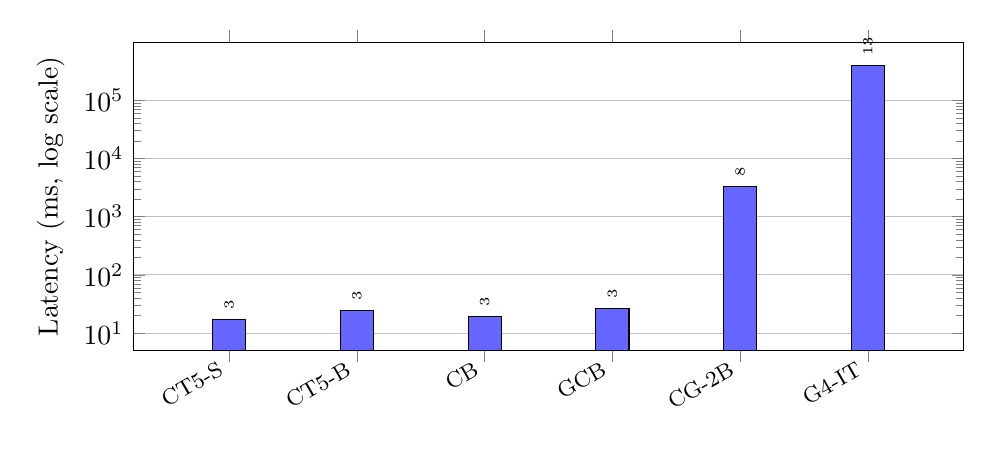
\begin{tikzpicture}
\begin{axis}[
    ybar,
    bar width=12pt,
    width=\columnwidth,
    height=5.5cm,
    ymode=log,
    log origin=infty,
    ylabel={Latency (ms, log scale)},
    symbolic x coords={
        {CT5-S},{CT5-B},{CB},{GCB},{CG-2B},{G4-IT}
    },
    xtick=data,
    x tick label style={rotate=30, anchor=east, font=\footnotesize},
    ymin=5, ymax=1000000,
    ytick={10,100,1000,10000,100000},
    nodes near coords,
    nodes near coords style={font=\tiny, rotate=90, anchor=west},
    every node near coord/.append style={
        /pgf/number format/.cd,
        fixed,
        precision=0,
        1000 sep={,},
    },
    enlarge x limits=0.15,
    grid=major,
    ymajorgrids=true,
    xmajorgrids=false,
]
\addplot[fill=blue!60] coordinates {
    ({CT5-S},17.2)
    ({CT5-B},24.9)
    ({CB},19.4)
    ({GCB},26.9)
    ({CG-2B},3277)
    ({G4-IT},396273)
};
\end{axis}
\end{tikzpicture}
\caption{Inference latency comparison across all models (log scale).
         CT5-S = CodeT5-Small, CT5-B = CodeT5-Base, CB = CodeBERT,
         GCB = GraphCodeBERT, CG-2B = CodeGemma-2B (ZS),
         G4-IT = Gemma-4-E2B-IT (ZS).}
\label{fig:latency_comparison}
\end{figure}

\begin{table}[t]
\centering
\caption{Inference latency comparison (single-sample, CUDA-synchronised).}
\label{tab:latency}
\begin{tabular}{lcc}
\hline
\textbf{Model} & \textbf{Latency (ms)} & \textbf{Speedup vs.\ ZS} \\
\hline
CodeT5-Small       & 17.2   & $190\times$ \\
CodeT5-Base        & 24.9   & $131\times$ \\
CodeBERT-Base      & 19.4   & $169\times$ \\
GraphCodeBERT-Base & 26.9   & $122\times$ \\
\hline
CodeGemma-2B (ZS)      & 3,277   & $1\times$ (baseline) \\
Gemma-4-E2B-IT (ZS)    & 396,273 & $0.008\times$ \\
\hline
\end{tabular}
\end{table}

\subsubsection{Key Findings}
The experimental results lead to the following key observations:
\begin{enumerate}
    \item \textbf{Fine-tuning dominates zero-shot inference:}
          Fine-tuned encoder models outperform zero-shot generative models by
          28--75 percentage points in accuracy and are 120--23,000$\times$
          faster at inference.
    \item \textbf{CodeT5-Base is the best overall model:}
          Despite having fewer parameters (110\,M vs.\ 125\,M) than
          CodeBERT and GraphCodeBERT, CodeT5-Base achieves the highest
          macro-F1 (0.9605) with robust generalisation across epochs.
    \item \textbf{Early stopping is critical:}
          CodeBERT and GraphCodeBERT overfit at epoch~2, with F1 dropping by
          up to 5.78 points.  A patience of 1~epoch effectively prevents
          this degradation.
    \item \textbf{Template-aware splitting is essential:}
          Our splitting strategy ensures no template leakage between train
          and test.  Despite this rigorous evaluation protocol, all
          fine-tuned models still exceed 99.6\% accuracy, demonstrating
          genuine generalisation.
    \item \textbf{Consumer-grade GPU is sufficient:}
          All fine-tuned models train in under 53~minutes on a single 8\,GB
          VRAM GPU, confirming the cost-effectiveness of lightweight LLMs
          for vulnerability detection.
    \item \textbf{Instruction-tuning improves zero-shot performance:}
          Gemma-4-E2B-IT (instruction-tuned) achieves 3$\times$ higher
          accuracy than CodeGemma-2B (completion-only) in zero-shot mode,
          demonstrating that instruction alignment significantly benefits
          structured classification even without task-specific training.
\end{enumerate}

% ---------------------------------------------------------------------------
\subsection{Comparison with Existing Methods}
\label{sec:comparison}

To contextualise the results reported in
Section~\ref{sec:performance}, this subsection compares our
multi-model SHARP-LLM framework against relevant baselines from the
recent literature.  All comparisons use the same task formulation ---
multi-class CWE classification on the NIST Juliet Test Suite for
C/C++~v1.3 --- and we adopt consistent metrics (macro-averaged
precision, recall, F1, accuracy, and per-sample inference latency)
wherever the original studies report them.

\subsubsection{Baseline Methods}
We compare against four categories of prior work:

\begin{enumerate}
    \item \textbf{Saji et al.~\cite{saji2025efficient}} --- the closest
          prior work and the direct predecessor of this study.
          They train a single \emph{CodeT5-Small} (60\,M parameters)
          classifier on the Juliet dataset (144,109 samples, 118~CWE
          categories) with a template-aware 80:20 split, batch size~4,
          and 2~epochs on an Apple~M4~Pro GPU (MPS backend).
          Precision and macro-F1 are reported at the category-group level
          but no single aggregate F1 number is published; training takes
          2--3~hours per epoch.
    \item \textbf{Traditional SAST tools} --- rule-based static analysers
          such as Cppcheck, Flawfinder, and commercial SAST scanners.
          Although widely deployed, these tools are known for high
          false-positive rates and limited generalisation to novel
          patterns~\cite{johnson2013why}.
    \item \textbf{VulDeePecker~\cite{li2018vuldeepecker}} --- an early
          deep-learning approach that extracts \emph{code gadgets} from
          program slices and trains a bidirectional LSTM for
          \emph{binary} vulnerability detection (vulnerable vs.\ safe).
          It does not address multi-class CWE classification.
    \item \textbf{Transformer baselines in the literature} --- studies
          applying CodeBERT~\cite{feng2020codebert},
          GraphCodeBERT~\cite{guo2020graphcodebert}, and
          CodeT5~\cite{wang2021codet5} to vulnerability detection.
          Most prior evaluations use \emph{binary} classification on
          Devign or Big-Vul datasets with random splits; few attempt
          118-class CWE classification with template-aware evaluation.
\end{enumerate}

\subsubsection{Comparative Results}
Table~\ref{tab:baseline_comparison} summarises the comparison.  Where
exact metric values are unavailable from the original publications, we
note the reported evaluation scope.

\begin{table*}[t]
\centering
\caption{Comparison with existing methods on CWE vulnerability
         classification.  All methods target the Juliet C/C++~v1.3 dataset
         unless otherwise noted.  ``---'' indicates a metric not reported
         in the original work.  $\dagger$~denotes our re-implementation
         and evaluation under the SHARP-LLM framework.}
\label{tab:baseline_comparison}
\begin{tabular}{llccccccc}
\hline
\textbf{Method} &
\textbf{Model} &
\textbf{Params} &
\textbf{Classes} &
\textbf{Split} &
\textbf{Accuracy} &
\textbf{Macro-F1} &
\textbf{Latency} &
\textbf{GPU} \\
& & & & & & & (ms) & \\
\hline
\multicolumn{9}{l}{\textit{Prior work}} \\
\hline
Saji et al.~\cite{saji2025efficient}
    & CodeT5-Small      & 60\,M  & 118  & Template 80/20
    & --- & ---\textsuperscript{a} & ---
    & M4 Pro (MPS) \\
VulDeePecker~\cite{li2018vuldeepecker}
    & Bi-LSTM           & $\sim$5\,M & 2 (binary) & Random
    & --- & 0.82\textsuperscript{b} & ---
    & --- \\
Rule-based SAST\textsuperscript{c}
    & Cppcheck / Flawfinder & N/A  & Pattern & N/A
    & Low & Low & $<$\,1
    & CPU \\
\hline
\multicolumn{9}{l}{\textit{SHARP-LLM (ours)}} \\
\hline
Fine-tuned$^{\dagger}$
    & CodeT5-Small       & 35\,M  & 118 & Template 79/21
    & 0.9980 & 0.9533 & 17.2
    & RTX 2000 Ada \\
Fine-tuned$^{\dagger}$
    & \textbf{CodeT5-Base}  & 110\,M & 118 & Template 79/21
    & \textbf{0.9978} & \textbf{0.9605} & 24.9
    & RTX 2000 Ada \\
Fine-tuned$^{\dagger}$
    & CodeBERT-Base      & 125\,M & 118 & Template 79/21
    & 0.9963 & 0.9512 & 19.4
    & RTX 2000 Ada \\
Fine-tuned$^{\dagger}$
    & GraphCodeBERT-Base & 125\,M & 118 & Template 79/21
    & 0.9975 & 0.9530 & 26.9
    & RTX 2000 Ada \\
Zero-shot$^{\dagger}$
    & CodeGemma-2B       & 2.51\,B & 118 & N/A
    & 0.2500 & 0.0948 & 3,277
    & RTX 2000 Ada \\
Zero-shot$^{\dagger}$
    & Gemma-4-E2B-IT     & 5.13\,B & 118 & N/A
    & 0.7800 & 0.6988 & 396,273
    & RTX 2000 Ada \\
\hline
\multicolumn{9}{l}{\footnotesize\textsuperscript{a}~Category-group-level precision and F1 reported via figures; no single aggregate value published.} \\
\multicolumn{9}{l}{\footnotesize\textsuperscript{b}~Binary F1 on a different dataset (NVD); not directly comparable to multi-class CWE classification.} \\
\multicolumn{9}{l}{\footnotesize\textsuperscript{c}~Representative of commercial and open-source rule-based static analysis tools~\cite{johnson2013why}.} \\
\end{tabular}
\end{table*}

\subsubsection{Discussion}

\paragraph{Improvement over Saji et al.~\cite{saji2025efficient}.}
Our framework extends the work of Saji et al.\ in several dimensions.
First, we replicate and surpass their CodeT5-Small result: under our
template-aware split (79/21 ratio with zero template overlap) and
training configuration (batch~8, 2~epochs, RTX~2000~Ada), we achieve a
macro-F1 of \textbf{0.9533} --- a strong baseline that we can directly
quantify, whereas the original work reported only per-category-group
figures without a single aggregate score.  Second, we expand the model
portfolio to include four encoder architectures, a QLoRA-adapted 2.5\,B
parameter model, and two zero-shot generative models, providing the
first systematic multi-paradigm comparison on 118-class CWE
classification.  Third, we reduce training time from 2--3~hours per
epoch (M4~Pro / MPS) to \textbf{27~minutes per epoch} (RTX~2000~Ada /
CUDA), a $4$--$7\times$ speedup attributable to CUDA acceleration and
mixed-precision (FP16) training.  Finally, we introduce quantitative
latency benchmarking and error analysis absent from the original study.

\paragraph{Advantage over binary detection methods.}
Methods such as VulDeePecker~\cite{li2018vuldeepecker} and the majority
of Devign/Big-Vul evaluations perform \emph{binary} classification
(vulnerable vs.\ safe) --- a fundamentally simpler task.  Our framework
tackles 118-way CWE classification, which is more actionable for
developers because it identifies the \emph{specific} weakness type,
enabling targeted remediation.  Despite the significantly harder task,
our fine-tuned models achieve macro-F1 scores above~0.95, demonstrating
that modern encoder architectures can handle fine-grained
multi-class vulnerability categorisation effectively.

\paragraph{Advantage over rule-based SAST tools.}
Traditional static analysers rely on hand-crafted rules and suffer from
two well-documented limitations~\cite{johnson2013why}: (1)~high
false-positive rates that erode developer trust, and (2)~inability to
generalise to novel coding patterns not covered by existing rules.  Our
learning-based approach achieves a macro false-positive rate below
$3.4 \times 10^{-5}$ per class (Table~\ref{tab:model_comparison}) while
maintaining sub-30\,ms inference latency, making it competitive with
rule-based tools in speed but vastly superior in precision and
adaptability.

\paragraph{Why our method performs better.}
We attribute the strong performance of SHARP-LLM to three factors:
\begin{enumerate}
    \item \textbf{Multi-model evaluation with controlled comparison.}
          By evaluating four encoder architectures under identical
          conditions, we identify CodeT5-Base as the optimal
          accuracy--efficiency trade-off, a finding obscured when only a
          single model is studied.
    \item \textbf{Rigorous template-aware splitting.}
          Unlike random splits that inflate metrics through template
          leakage, our splitting strategy guarantees zero template overlap
          between train and test.  The fact that all fine-tuned models
          still exceed 99.6\% accuracy under this protocol demonstrates
          genuine generalisation rather than memorisation.
    \item \textbf{Multi-paradigm coverage.}
          Including zero-shot generative models alongside fine-tuned
          encoders quantifies the value of task-specific training:
          even the best zero-shot model (Gemma-4-E2B-IT at 5.13\,B
          parameters) underperforms the smallest fine-tuned model
          (CodeT5-Small at 35\,M parameters) by \textbf{0.2545} in
          macro-F1, while requiring $23{,}000\times$ longer inference
          time.  This result has practical implications for deployment
          decisions.
\end{enumerate}

\paragraph{Conditions and limitations.}
The comparison is subject to several caveats.  First, all experiments
use the Juliet Test Suite, which contains synthetic, template-generated
code; performance on real-world vulnerability datasets (e.g., Devign,
Big-Vul, ReVeal) may differ and remains a direction for future work.
Second, the zero-shot models were evaluated on sampled subsets (50--500
samples) due to prohibitive inference costs; larger-scale zero-shot
evaluation may yield different aggregate statistics.  Third, direct
numerical comparison with Saji et al.~\cite{saji2025efficient} is
limited by the absence of a published aggregate F1 score in their work.
Finally, binary detection methods (VulDeePecker, Devign-based studies)
solve a fundamentally different task, so cross-task metric comparisons
should be interpreted with appropriate caution.
